\documentclass[ngerman]{scrartcl} 

\KOMAoptions{fontsize=12pt, paper=a4}
\KOMAoptions{DIV=11}
\usepackage[utf8]{inputenc}		% Direkte Eingabe von ä usw.
\usepackage[T1]{fontenc}               	% Font Kodierung für die Ausgabe
\usepackage{babel}			% Verschiedenste sprach-spezifische Extras
\usepackage[autostyle=true]{csquotes}	% Intelligente Anführungszeichen
\usepackage{amsmath}		% Mathematischer Formelsatz mit zusätzlichen mathematischen Schriften und Symbolen
\usepackage{amssymb}		% Mathematischer Formelsatz mit zusätzlichen mathematischen Schriften und Symbolen
\usepackage{physics}			% Differentialgleichungen
\usepackage{listings}			% Zum Einbinden von Programmcode verwenden wir das listings-Paket
\usepackage[dvipsnames]{xcolor}	% um Elemente von Befehlen farblich zu unterstützen
\usepackage[varg]{txfonts}             	 % Schönere Schriftart
\usepackage{graphicx}		% Paket um externe Graphiken einzufügen
%\RequirePackage[backend=biber, style=numeric]{biblatex} % Literaturverzeichnis
\usepackage{hyperref} 		% um klickbare Elemente in Ihrem PDF-Ausgabedokument zu erzeugen
%\RequirePackage[all]{hypcap} 		% ergänzend zu hyperref
\usepackage{siunitx}			% Intelligentes Setzten von Zahlen und Einheiten
\usepackage{enumitem}		% Aufzählungsarten
\usepackage{fancyhdr}
\usepackage{float}			% Bild genau an der gewünschten Stelle [H] einfügen, 								% \begin{figure}[H]		\includegraphics[...]{{file name}}		\end{figure} 

\setlength\parindent{0pt} 		% Sets paragraph indentation to 0

\lstset{				% Deutsche Umlaute
	basicstyle=\ttfamily,    
	literate={~} {$\sim$}{1} 	% set tilde as a literal
	{ö}{{\"o}}1
	{ä}{{\"a}}1
	{ü}{{\"u}}1
	{ß}{{\ss}}1
	{Ö}{{\"O}}1
	{Ä}{{\"A}}1
	{Ü}{{\"U}}1
}
\lstset{
	numbers=left, 				% Line numbering
	numberstyle=\footnotesize, 			% Size of numbers
	basicstyle=\ttfamily\small, 			% Style and Size of Text
	backgroundcolor=\color{White}, 		% Background Color
	language=Python, 				% Language of Code
	commentstyle=\color{Maroon}, 			% Color and Style of Comments
	stringstyle=\color{OliveGreen}, 			% Color of Strings
	showstringspaces=false,
	morekeywords={import,from,class,def,for,while,if,is,in,elif,else,not,and,or,print,break,continue,return,True,False,None,access,as,del,except,exec,finally,global,import,lambda,pass,print,raise,try,assert}, 												% Definition of new keywords that will be highlighted
	keywordstyle=\color{RoyalBlue}			% Color and Style of Keywords
}


\pagestyle{fancy}
\fancyhf{}
\rhead{Ben Karcher, Annika Hoverath}
\lhead{Computerphysik - Abgabe 2}
\rfoot{Seite \thepage}

\title{Computerphysik - Abgabe 2}
\date{22.05.2020}

\begin{document}

\thispagestyle{fancy}

\section{H.4 Periodische Schwingungen}
In dieser Aufgabe betrachten wir zunächst einen gedämpften harmonischen Oszillator $x(t)$. Dieser wird in vektorieller Form durch die Bewegungsgleichungen
\begin{align}
\vec{f}(t)=\vec{\dot{x}}=\left(\begin{array}{c} \dot{x}^{(1)} \\ \dot{x}^{(2)} \end{array}\right) = \left(\begin{array}{c} x^{(2)} \\ -\omega_{0}^{2}x^{(1)} - 2\gamma x ^{(2)}\end{array}\right)
\end{align} 
beschrieben. Die Anfangsbedingungen sind so gewählt, dass sich der Oszillator zum Zeitpunkt $t=0$ am Ort $x_{0}$ mit der Anfangsgeschwindigkeit $v_{0}$ befindet. Dabei bewegt sich der harmonische Oszillator im Uhrzeigersinn, also gilt $\omega_{0}>0$. Da der harmonische Oszillator gedämpft wird, ist der Dämpfungsfaktor größer als 0 ($\gamma>0$). 
\subsection{H.4 1 gedämpfte Schwingungen}
In dieser Teilaufgabe approximieren wir die Differentialgleichung und suchen die stabilen Orte der Funktion um Aussagen über die beiden kritsich gedämpften Schwingungen zu machen. Dazu wenden wir zunächst das Euler-Cauchy-Verfahren an. Mit diesem Verfahren löst man numerisch gewöhnliche Differentialgleichungen, denn man approximiert den Graphen durch eine Polynomfunktion. Ausgehend von der Ausgangssteigung an der Stelle $x_{0}$ iteriert man durch die folgenden Funktionswerte $y_{i+1}$, die eine Steigung im Intervall 
\begin{equation} \vec{x}_{i+1}=\vec{x}_{i}+h\vec{f}(t,\vec{x}_{n}) \end{equation} 
zurücklegen. Dabei wird die Steigung durch eine Sekante zwischen den beiden Werten angenommen. Somit setzt sich die Polynomfunktion aus vielen kleinen Geradenstücken zusammen. Je kleiner man die Steilstücke $h$ wählt, desto genauer approximiert die Polynomfunktion die Differentialgleichung. Diese hohe Genauigkeit hat jedoch den Nachteil, dass es viel Rechenkapazität, also Zeit braucht. \newline 
Bringen wir nun die beiden Gleichungen in die folgende Vergrößerungsmatrix:
\begin{align}
M=\left(\begin{array}{cc} 1 & h \\ -h\omega_{0}^{2} & 1-2h\gamma \end{array}\right)
\end{align}
Die charakteristischen Eigenwerte $\lambda_{1,2}$ sind: $\lambda_{1,2}=-h\gamma+1\pm\sqrt{\gamma^2-\omega^2_0}$
Nun stellt sich die Frage, an welchen Orten $x(t)$ sich der Oszillator in einem stabilen oder instabilen Zustand befindet. Dieses Stabilitätsproblem versuchen wir nun im Folgenden zu lösen. Dafür machen wir eine Fallunterscheidung der Dämpfung. Es gibt drei Fälle, den überkritischen Fall ($\gamma < \omega_0$), den kritischen Fall ($\gamma = \omega_0$) und den unterkritischen Fall ($\gamma > \omega_0$). Um ein stabiles Verfahren zu haben, muss der maximale Betrag der Eigenwerte kleiner als 1 sein. Somit erhält man mit der Gleichung der Eigenwerte zwei Möglichkeiten: 
\begin{itemize}
 	\item[$\gamma > \omega_0$] Für diesen Fall gilt dann  \begin{equation*}  |\lambda_{1,2}| = |-h\gamma + 1 \pm h\sqrt{\gamma^2-\omega_0^2}  \end{equation*}  Dieser Fall ist nur sehr wenig stabil, denn es gilt: $\lim_{h \to 0} |\lambda_{1,2}| \rightarrow 1$.
	\item[$\gamma = \omega_0$] Dieser Fall lässt sich stabil simulieren. Es gilt:  \begin{equation*}  |\lambda_{1,2}| = | 1 - h\gamma|  \end{equation*}  Der Fall ist stabil, wenn $|h| < \frac{2}{\gamma}$, denn dann gilt $|\lambda_{1,2}| < 1$.
	\item[$\gamma < \omega_0$] Dieser Fall ist ebenfalls nicht stabil implementierbar, denn es gilt:  \begin{equation*}  |\lambda_{1,2}| = |-h\gamma + 1 \pm h\sqrt{\gamma^2 - \omega_0^2}|  \end{equation*}  Dabei gilt dann $\lim_{h \to 0} |\lambda_{1,2}| \rightarrow 1$. Somit ist auch dieses Verfahren nur gering stabil.
\end{itemize}
Daraus schlussfolgern wir, dass das Euler-Cauchy-Verfahren nur bei überkritischer Dämpfung stabil sein kann mit $h<\frac{2}{\gamma}$. Somit sehen wir, dass wir nicht jeden Fall der gedämpften Schwingung mit dem Euler-Cauchy-Verfahren simulieren bzw. implementieren können.
\begin{figure}[htbp]
	\centering
	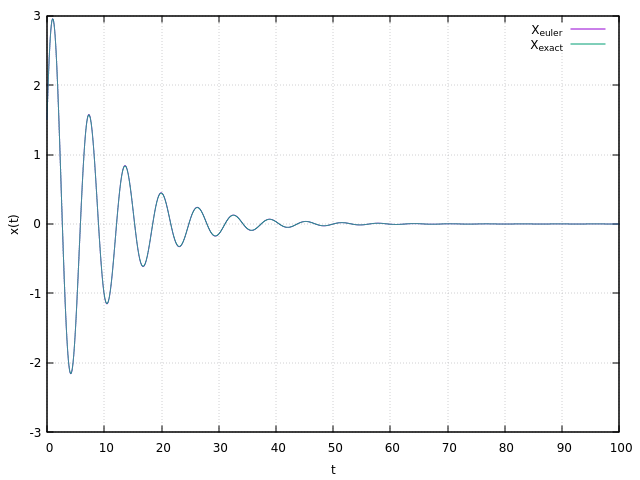
\includegraphics[width=0.45\textwidth]{euler}
	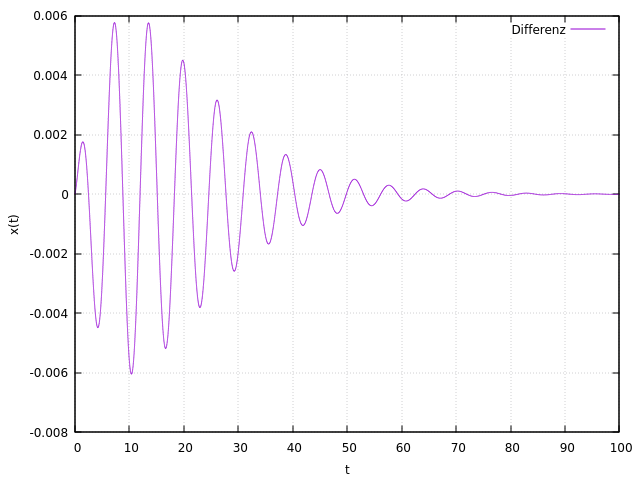
\includegraphics[width=0.45\textwidth]{euler_fehler}
	\caption[$f{ext}$]{Hier ist das resultat des Euler verfahrens dargestellt.}
	\label{fig:euler}
\end{figure}
\subsection{H.4 2 Runge-Kutta-Verfahren 4. Ordnung}
In dieser Aufgabe implementieren wir das Runge-Kutta-Verfahren für die 4. Ordnung, um die Differentialgleichung zu lösen. Dies ist eine Verbesserung des Euler-Cauchy-Verfahrens und ist ähnlich zu der Taylor-Reihenentwicklung, nur dass die höheren Ordnungen über der zweiten Ordnung mit in die Funktion einfließen. Nun wird die Steigung aber nicht aus einer Geraden ermittelt, sondern man verwendet vier Hilfssteigungen, wobei zwei der vier Steigungen doppelt stark gewichtet werden. Die Steigung ergibt sich aus $m=\frac{m_{0}+2 m_{1}+2 m_{2}+m_{3}}{6}$, wobei $m_{0}$ die Steigung am Ausgangspunkt A ist, die man erhält, wenn man A in die obige Differentialgleichung einsetzt ($m_{0}=\dot{x}(t=0,x_{0})$). Die Steigung $m_{1}$ (doppelt gewichtet) ist durch die Steigung $m_{0}$ festgelegt und verläuft zu einem Hilfspunkt $P_{1}$, der sich auf der Hälfte des Weges zum Ziel befindet ($P_{1}=x(t+\frac{h}{2})$). Für die doppelt gewichtete Steigung $m_{2}$ führen wir einen weiteren Hilfspunkt $P_{2}$ ein, der, genauso wie $P_{1}$, bei der Hälfte der Strecke zum Ziel liegt, aber nun eine andere Steigung $m_{2}$ verursacht. Zu guter Letzt ergibt sich $m_{3}$, indem die Gerade vom Punkt A über den Punkt $P_{2}$ zum Zielzeitpunkt $t+h$ verläuft. Zusammen ergeben die vier gewichteten Hilfssteigungen nach obiger Formel die Steigung. Um das Verfahren verifizieren zu können, müssen wir zunächst einmal die analytische Lösung des Problems bestimmen und untersuchen anschließend die Differenz der beiden Lösungen. Zunächst machen wir einen allgemeinen Ansatz:
\begin{equation} x(t)=Ae^{\lambda_{1}t} + Be^{\lambda_{2}t}\end{equation}
\begin{equation}\lambda_{1,2}= - \gamma \pm i\tilde{\omega}\end{equation}
\begin{equation}\tilde{\omega_0}=\sqrt{\gamma^2 - \omega^2_0}\end{equation}
Schlussendlich erhalten wir mit den Anfangsbedingungen $x(0)=x_0$ und $\dot{x}(0)=v_0$ die analytische Funktion:
%\begin{equation} x(t)=e^{-\gamma t}\left[x_0 \cos(\tilde{\omega}t) + \frac{v_0 + x_0 \gamma}{\tilde{\omega}} \sin(\tilde{\omega}t)] \end{equation}
Vergleicht man die so erhaltene Lösung mit der exakten Lösung, so sieht man, dass die erhaltene Lösung für kleine Zeiten $t$ sehr gut übereinstimmt. Dies bedeutet, dass das Runge-Kutta-Verfahren eine sehr gute Approximation für die Differentialgleichung eines harmonisch gedämpften Oszillators darstellt. Auch für größere Zeiten läuft dieses Verfahren ebenfalls sehr gut. Die Differenz der beiden Lösungen befindet sich etwa in der Größenordnung von $10^-12$. Dies verifiziert das Runge-Kutta-Verfahren für die 4. Ordnung.
\begin{figure}[htbp]
	\centering
	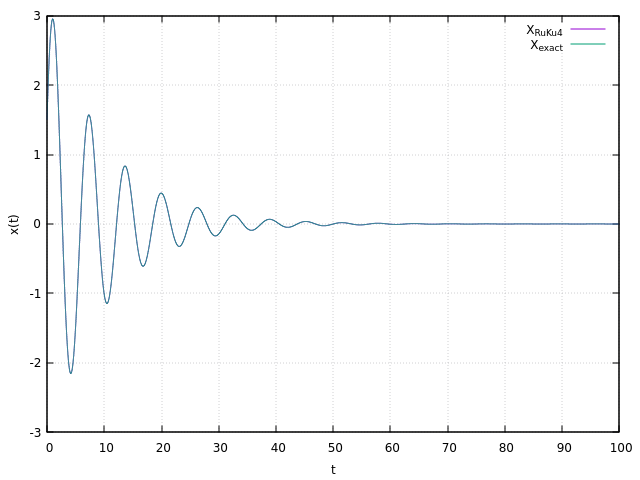
\includegraphics[width=0.45\textwidth]{ruku}
	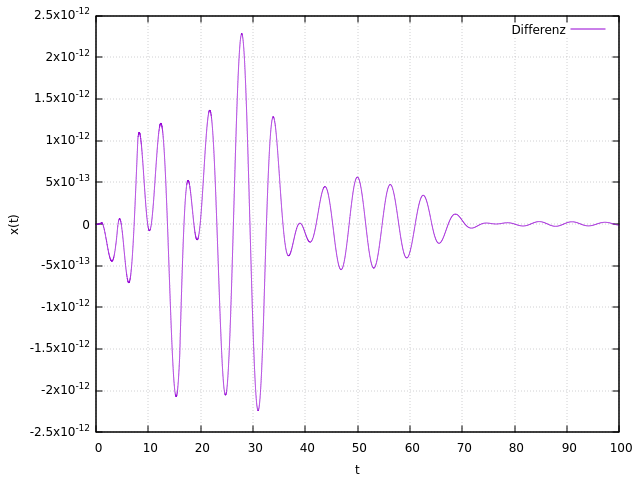
\includegraphics[width=0.45\textwidth]{ruku_fehler}
	\caption[$f{ext}$]{Hier ist das resultat des RK4 verfahrens dargestellt.}
	\label{fig:euler}
\end{figure}
\subsection{H.4 3 Korrektheit von RK4}
Wir haben nun in der Aufgabe H.4 2 gesehen, dass die RK4 die DGL sehr gut approximiert. Im Anschluss betrachten wir eine lineare DGL der Form
\begin{equation}
\frac{d}{dt}y(t)=F \cdot y(t) , F=const
\end{equation}
Mit dieser Gleichung werden wir zeigen, dass die RK4 zur Ordnung 4 für den Zeitschritt $h$ erfüllt ist. Wir taylorn die Funktion $\vec{y}(t)$. Einen einzelnen Zeitschritt $h$ können wir durch die Formel: 
\begin{equation} \vec{y}(t+h) = \vec{y}(t) + h\frac{d\vec{y}}{dt}(t) + \frac{h^2}{2}\frac{d^2\vec{y}}{dt^2} + \frac{h^3}{6}\frac{d^3\vec{y}}{dt^3} + \frac{h^4}{24}\frac{d^4\vec{y}}{dt^4} + \mathcal{O}(h^5) \end{equation} ausdrücken. Die DGL ist linear zu ihren linearen Koeffizienten, weshalb wir die Ableitungen schreiben können als:
\begin{equation*} \frac{d^n\vec{y}(t)}{dt^n} = F^n*\vec{y}(t) \end{equation*} wobei $F$ eine Matrix beschreibt. Aus der DGL lässt sich die Matrix bestimmen zu: \begin{equation*} F = \begin{pmatrix} 0 & 1 \\ -\omega_0^2 & -2\gamma \end{pmatrix} \end{equation*}
Nun wenden wir das Runge-Kutta-Verfahren an. Mit der Iteration über die einzelnen Zeitdifferenzen $h$ erhalten wir durch Umformung: \begin{equation} \vec{y}(t+h) = \vec{y}(t) + \frac{1}{6}[\vec{m_0} + 2\vec{m_1} + 2\vec{m_2} + \vec{m_3}] \end{equation} Die vier Steigungen ergeben sich durch: 
\begin{align*} \vec{m_0} &= h\vec{f}(t, \vec{y(t)}) \\  \vec{m_1} &= h\vec{f}(t+h/2, \vec{y(t)}+\vec{m_0}/2) \\  \vec{m_0} &= h\vec{f}(t+h/2, \vec{y(t)}+\vec{m_1}/2) \\  \vec{m_3} &= h\vec{f}(t+h , \vec{y(t)} + \vec{m_2}) \end{align*}
Wenn wir nun in diese Terme unsere lineare DGL $\vec{f}(t, \vec{y(t)}) = F*\vec{y(t)}$ einsetzen, die Terme umformen und ineinander einsetzen, ergeben sich daraus die folgenden Gleichungen: \begin{align}  \vec{m_0} &= hF*\vec{y(t)} \\  \vec{m_1} &= hF*\left(\vec{y(t)} + \frac{h}{2}F\vec{y(t)}\right) \\  \vec{m_2} &= hF*\left(\vec{y(t)} + \frac{h}{2}F*\left(\vec{y(t)} + \frac{h}{2}F*\vec{y(t)}\right)\right) \\  \vec{m_3} &= hF*\left(\vec{y(t)} + hF*\left(\vec{y(t)}+\frac{h}{2}F*\left(\vec{y(t)} + \frac{h}{2}F*\vec{y(t)}\right)\right)\right) \end{align}
Zum Schluss setzen wir nun diese Steigungen in die Iterationsvorschrift des Runge-Kutta-Verfahrens ein. Daraus folgt: \begin{equation} \vec{y}(t+h) = \vec{y}(t) + hF*\vec{y}(t) + \frac{h^2}{2}F^2*\vec{y}(t) + \frac{h^3}{6}F^3*\vec{y}(t) + \frac{h^4}{24}F^4*\vec{y}(t) \end{equation} Diese Formel beweist, dass das Verfahren von RK4 bis zur Ordnung $\mathcal{O}(h^5)$ mit der obigen analytischen Lösung übereinstimmt. \newline
Im Anschluss führen wir bei der ersten DGL die Stabilitätsanalyse durch. Aus der Vergrößerungsmatrix $M$ lesen wir eine Art Taylorfunktion: \begin{equation*} M = hF + \frac{h^2}{2}F^2 + \frac{h^3}{6}F^3 + \frac{h^4}{24}F^4 \end{equation*}
Mit den Werten von $\omega_{0}=1$ und $\gamma=0.1$ sowie $x_{0}=1.5, v_{0}=2.75$  ergibt sich die Vergrößerungsmatrix \begin{equation} M = \begin{pmatrix} -\frac{h^2}{2}+\frac{h^3}{30}+\frac{h^4}{25} & h-\frac{0,2h^2}{2} - \frac{0,96h^3}{6} + \frac{0,392h^4}{24}\\  -h++\frac{0,2h^2}{2} + \frac{0,96h^3}{6} - \frac{0.392h^4}{24} & -0,2h-\frac{0,96h^2}{2} + \frac{0.392h^3}{6} + \frac{0.8816h^4}{24}  \end{pmatrix}\end{equation}
Die charakteristischen Eigenwerte $\lambda_{1,2}$ errechnet uns Mathematica zu: \begin{align*}  \lambda_{1,2} &=0.000868056 h [-564.48 h-115.2+44.1984 h^3+56.832 h^2 \\  & \pm \sqrt{-350.501 h^6+6866.97 h^5-29342.3 h^4-84961.2 h^3+407288.h^2+262767. h-1.31383\times 10^6}]  \end{align*} Wir sehen, dass wenn $lim {h \to 0}$, die Eigenwerte zu 0 verschwinden. Daraus schlussfolgern wir, dass bei sehr klein gewählten $h$ das RK4-Verfahren stabil ist und die analytische Funktion approximiert. Den Spektralradius $\rho$, auch Spur genannt, erhält man mit der Formel $\rho(F):=max_{1 \leq i  \leq n} |\lambda_{1,2}|$. Leider konnten wir in Mathematika die Ungleichung $|\lambda_{1,2}| < 1$ nicht lösen, weshalb wir nun leider keinen konkreten Wert erhalten haben.
\section{H.5 Kopplung an ein externes Feld}
Im Folgenden nehmen wir an, dass der Oszillator an ein externes Feld gekoppelt sein. Deswegen wirkt eine zusätzliche Kraft $f(t)$ auf ihn. 
\subsection{H.5 1 Spezialfall mit einer Cosinus förmigen Kraft}
Zunächst nehmen wir eine vereinfachte Kraft $f(t)=\alpha cos(\omega t)$ an. Diese externe Kraft simulieren wir, indem sie das exteren Feld anregt. Somit erhalten wir die neue DGL der Form:
\begin{equation} \frac{d^2x}{dt^2}(t)=\omega^2_0 x(t) -2\gamma \frac{dx}{dt}(t)+\alpha cos(\omega t) \end{equation}
Man erkennt schnell, dass sich diese DGL aus einer homogenen DGL und einem inhomogenen Teil zusammensetzt. Um die homogene DGL zu lösen, wählen wir den allgemeinen Ansatz: $x_{hom}(t)=e^{-\gamma t}[A cos(\tilde{\omega}t)+B sin(\tilde{\omega}t)]$. Die inhomogene DGL lässt sich durch die Funktion $x _{inhomogen}(t)=C cos{\omega t}+D sin{\omega t}$ konstruieren. Zuerst lösen wir unsere inhomogene DGL, wobei C und D die DGL erfüllen müssen. Für die beiden Platzhalter erhalten wir: 
\begin{equation*} C=\frac{\alpha(\omega^2_0 - \omega^2)}{(\omega_0-\omega)+4\gamma\omega}\end{equation*}\begin{equation*}D=\frac{2\gamma\alpha\omega}{(\omega_0-\omega)+4\gamma\omega} \end{equation*} Anschließend lösen wir den Ansatz für die homogene DGL, wobei die Faktoren A und B die Anfangsbedingungen der DGL natürlich erfüllen müssen. Die ermittelten Werte lauten: 
\begin{equation*} A=x_0-\frac{\alpha(\omega_0-\omega}{(\omega_0-\omega)+4\gamma\omega} \end{equation*}\begin{equation*} B=\frac{v_0}{{\tilde{\omega}}+\frac{\gamma A}{\tilde{\omega}}}-\frac{2\gamma\alpha\omega}{((\omega_0-\omega)+4\gamma\omega)\tilde{\omega}} \end{equation*} 
Es gilt, wie oben, $\tilde{\omega}= \sqrt{\gamma-\omega_0}$.

\subsection{H.5 2 Überprüfung mit der exakten Lösung}
Nun überprüfen wir in unserem Programm, analog zu der obigen Aufgabe, die Genauigkeit des Verfahrens.  Wir verwenden wieder dieselben Parameter wobei $\alpha=0.5$ und $\omega=1.5$ zusätzlich dazu kommen. Hier sehen wir ebenfalls, dass die Genauigkeit bei sehr kleinen Zeiten sehr groß ist. Bei größeren Zeiten $t$ liegen die Ungenauigkeiten ebenfalls wieder in der Größenordnung von etwa $10^{-10}$. Daraus schlussfolgern wir, dass dieses Verfahren ebenfalls für erzwungene Schwingungen gut anwendbar ist. Also können wir in der nächsten Aufgabe auch eine Frequenzanalyse für viele Perioden durchführen.
\begin{figure}[htbp]
	\centering
	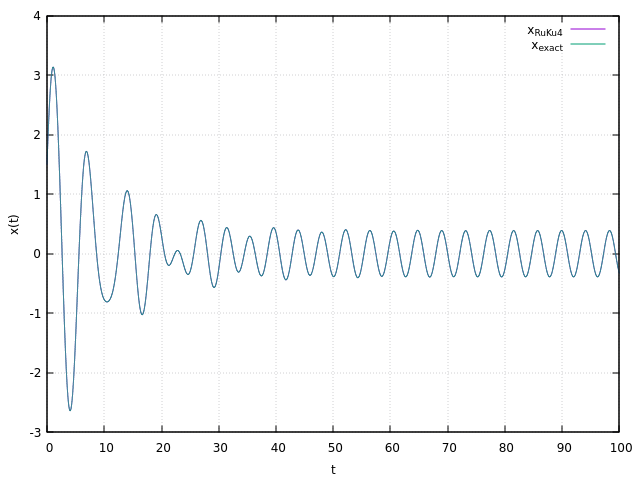
\includegraphics[width=0.45\textwidth]{ruku_extern}
	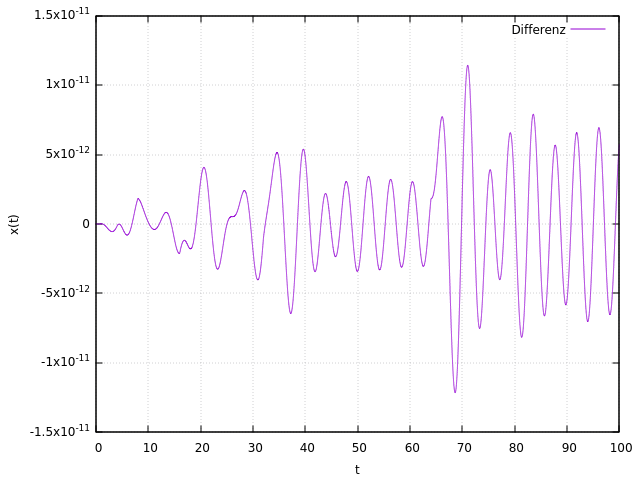
\includegraphics[width=0.45\textwidth]{ruku_extern_fehler}
	\caption[$f{ext}$]{Hier ist das resultat des RK4 verfahrens dargestellt.}
	\label{fig:euler}
\end{figure}
\section{H.6 Tune in}
Nun betrachten wir den Fall, dass wir eine externe, unbekannte Kraft $f_{ext}$ haben, die an unseren harmonischen Oszillator gekoppelt ist. $f_{ext}$ simuliert eine Überlagerung von einem Signal mit einem Rauschen, abhängig von ihrer Frequenz. 
\subsection{H.6 1 Erweiterung mit $f_{ext}$}
Zu aller erst erweitern wir die Funktion aus Aufgabe H.4 mit unserer externen Kraft $f_{ext}$. Die vorherige DGL ändert sich zu: \begin{equation}  \frac{d^2x}{dt^2}(t) = -\omega_0^2x(t) - 2\gamma\frac{dx}{dt}(t) + \alpha\cos(\omega t)  \end{equation}. Die neue sinusförmige, abfallende Bahnkurve überwiegt zunächst bei ihrer Schwingung. Doch bei einer Zeit von etwa $t=7,5[s]$ ist diese Schwingung so sehr abgefallen, dass nun die externe Kraft bei der Schwingung überwiegt und nun diese Schwingung zwingt mit der „Eigenfrequenz“ des externen schwingenden Feldes mitzuschwingen. Diese erzwungene Schwingung ist nun alles andere als eine gedämpfte, harmonische Schwingung. 
\subsection{H.6 2 gemittelte Leistung}
Nun berechnen wir numerisch, ausgehend von der momentanen Leistung $P(t) = f_{ext}(t)\dot{x}(t)$,  die durchschnittliche Leistung $\overline{P(t)} = \frac{1}{T}\int_{t_1}^{t_1+T}P(t)dt$, die innerhalb einer Periode gebraucht wird. Wir wissen, dass eine Periode $T$ physikalisch definiert ist als $T = 2\pi\omega_0$. Wir haben in der Aufgabe H5.2 bereits gezeigt, dass das RK4-Verfahren für große $t$ ebenfalls stabil ist. Somit nutzen wir diese Kenntnis und können nun die durchschnittliche Leistung über mehrere Perioden bestimmen. Das Integral lösen bzw. nähern wir durch das Trapez-Verfahren. In der folgenden Abbildung ist die durchschnittliche Leistung für die ersten zwölf Perioden mit der Kreisfrequenz $\omega_0=1 [s^{-1}]$ dargestellt. 
\subsection{H.6 3 Scan in $\omega_0$}
In dieser aller letzten Teilaufgabe führen wir nun den Scan in $\omega_0$ durch. Anschließend bestimmen wir über 60 Perioden  die durchschnittliche Leistung $\overline{P(t)}$, die durchschnittliche Leistung $\overline{P(\omega_0)}$, den Mittelwert und den Standardfehler. Hierbei verwenden wir die Parameter $\gamma=0,1$ und die Schrittweite $h=0,001$. Im Scan variieren wir $\omega_0$, sodass $\omega_0$ Werte zwischen 1 und 3 annimmt.  
Wir sehen drei ausgeprägte Peaks bei verschiedenen Eigenfrequenzen $\omega_0$. Daraus können wir auf die drei Eigenfrequenzen der externen, anregenden Schwingung $f_{ext}(t)$  schließen. Dieses Verfahren ist quasi eine Fourieranalyse. Sie zerlegt eine (überlagerte) Schwingung anteilmäßig in ihre Eigenfrequenzkomponenten. Wir erhalten diesen Graphen, da die Leistung maximal wird, wenn die Differenz zwischen der Anrege- und Eigenfrequenz sehr klein wird. Somit haben wir unsere unbekannte Funktion in ihre Einzelfrequenzanteile zerlegt und konnten darüber Aussagen über die, uns unbekannte, Funktion machen.

\begin{figure}[htbp]
	\centering
	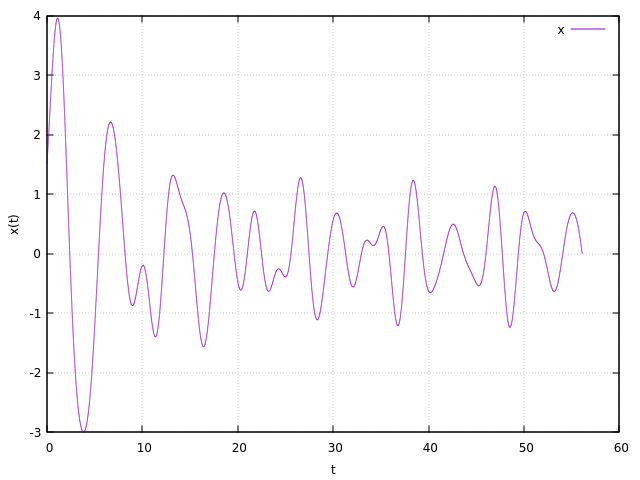
\includegraphics[width=0.7\textwidth]{fext_x}
	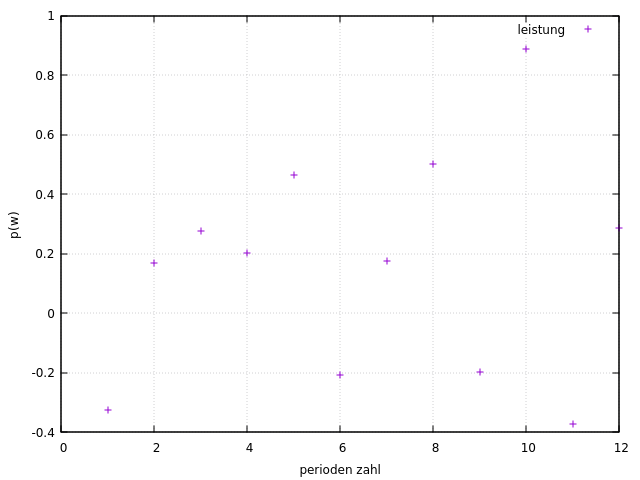
\includegraphics[width=0.7\textwidth]{fext_leistung}
	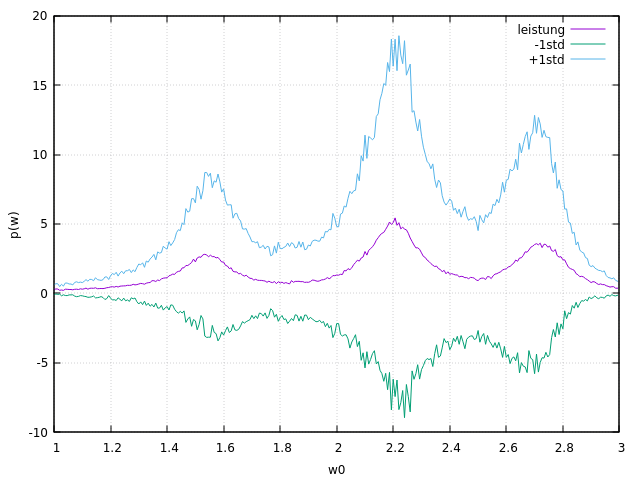
\includegraphics[width=0.7\textwidth]{fext_scan}
	\caption[$f{ext}$]{Hier wird die resultierende Bahn x(t) dargestelt sowie die Leistung von fext.}
	\label{fig:euler}
\end{figure}

\end{document}

